\chapter{Geometry and Measurement: Part I}

The SAT math section includes topics in Geometry as well as Algebra. The equations that are given on the SAT all pertain to Geometry and are listed below. Know the equations that are given so as not to work on memorizing them.

\bigskip
\headertitle{SAT Math Given Equations}

\vspace{-0.5em}
\begin{center}
\begin{tabularx}{\textwidth}{*4{@{}>{\centering\arraybackslash}X}}
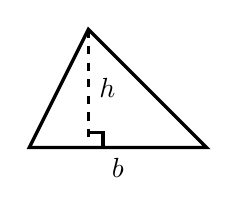
\begin{tikzpicture}[scale=0.75, very thick]
\draw (0,0) -- (1,2) -- (3,0) -- node[midway, below] {$b$} cycle;
\draw[dashed] (1,2) -- node[midway, right] {$h$} (1,0);
\draw (1,0.25) -- (1.25,0.25) -- (1.25,0);
\end{tikzpicture}
&
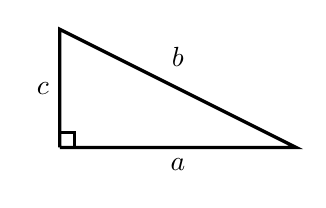
\begin{tikzpicture}[scale=0.75, very thick]
\draw (0,0) -- node[midway, below] {$a$} (4,0) -- node[midway, label=$b$] {} (0,2) -- node[midway, left] {$c$} (0,0);
\draw (0,0.25) -- (0.25, 0.25) -- (0.25,0);
\end{tikzpicture}
&
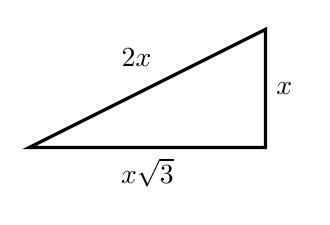
\begin{tikzpicture}[scale=0.75, very thick]
\draw (0,0) -- node[midway, below] {$x\sqrt{3}$} (4,0) -- node[midway, right] {$x$} (4,2) -- node[midway, left, label=$2x$] {} cycle;
\end{tikzpicture}
&
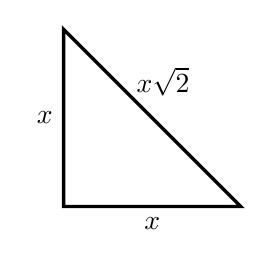
\begin{tikzpicture}[scale=0.75, very thick]
\draw (0,0) -- node[midway, below] {$x$} (3,0) -- node[midway, right, label=$x\sqrt{2}$] {} (0,3) -- node[midway, left] {$x$} cycle;
\end{tikzpicture}\\
$A=\frac{1}{2}bh$ & $c^2=a^2+b^2$ & \multicolumn{2}{c}{Special Right Triangles}
\end{tabularx}

\vfill
\begin{tabularx}{0.8\textwidth}{*2{@{}>{\centering\arraybackslash}X}}
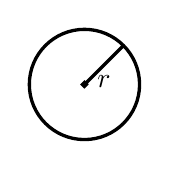
\begin{tikzpicture}[scale=0.7, very thick]
\draw (0,0) circle (1cm);
\draw[fill] (0,0) circle (1pt) -- node[midway, below] {$r$} (0.707, 0.707);
\end{tikzpicture}
&
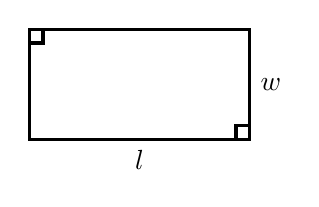
\begin{tikzpicture}[scale=0.7, very thick]
\draw (0,0) -- node[midway, below] {$l$} (4,0) -- node[midway, right] {$w$} (4,2) -- (0,2) -- cycle;
\draw (0,1.75) -- (0.25,1.75) -- (0.25,2);
\draw (3.75,0) -- (3.75,0.25) -- (4,0.25);
\end{tikzpicture}\\
$A=\pi r^2$ & \multirow{2}{*}{$A=lw$}\\
$C=2\pi r$ & \\
\end{tabularx}

\vfill
\begin{tabularx}{0.8\textwidth}{*2{@{}>{\centering\arraybackslash}X}}
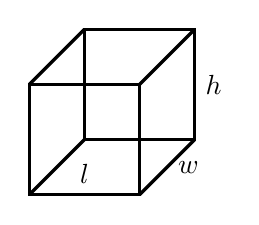
\begin{tikzpicture}[scale=0.7, very thick]
\draw (0,0) -- node[midway, above] {$l$} (2,0) -- (2,2) -- (0,2) -- cycle;
\draw (1,1) -- (3,1) -- node[midway, right] {$h$} (3,3) -- (1,3) -- cycle;
\draw (0,0) -- (1,1);
\draw (2,0) -- node[midway, right] {$w$} (3,1);
\draw (2,2) -- (3,3);
\draw (0,2) -- (1,3);
\end{tikzpicture}
&
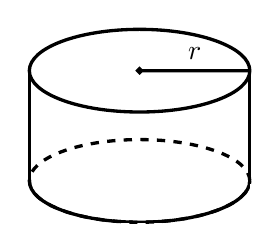
\begin{tikzpicture}[scale=0.7, very thick]
\draw (0,0) ellipse (2cm and 0.75cm);
\draw[fill] (0,0) circle (1pt) -- node[midway, above] {$r$} (2,0);
\draw (-2,0) -- (-2,-2);
\draw (2,0) -- (2,-2);
\draw[dashed] (0,-2) ellipse (2cm and 0.75cm);
\clip (-2,-2) rectangle (2,-2.75);
\draw (0,-2) ellipse (2cm and 0.75cm);
\end{tikzpicture}\\
$V=lwh$ & $V=\pi r^2h$
\end{tabularx}
\end{center}

\vfill
The number of degrees of arc in a circle is 360.

The sum of the measures in degrees of the angles of a triangle is 180.